\chapter{Requisiti specifici}
In questo capitolo verranno illustrati le funzionalità identificate dal capitolato d'appalto \textit{GDP-Gathering Detection Platform}. 
\section{FC1: Acquisizione dati}
L'acquisizione dei dati avverrà in tre fasi descritte di seguito.
\subsection{FC1.1: Acquisizione con java}
\begin{itemize}
	\item \textbf{Descrizione}: attraverso il linguaggio Java si creerà un programma che preleva informazioni da sorgenti esterne e le invia al server.
	\item \textbf{Linguaggio di programmazione}: Java.
	\item \textbf{Input}: i dati forniti saranno prelevati da siti con live-feed di webcam di Roma e simulatori di spostamenti di persone.
	\item \textbf{Output}: i dati resteranno immutati.
	\item \textbf{Risposta ad errori}: nel caso di mancanza di risposta dai siti con live-feed il programma si bloccherà ed invierà un segnale di errore al server.
\end{itemize}
\subsection{FC1.2: Creazione database}
\begin{itemize}
	\item \textbf{Descrizione}: attraverso lo studio dei tipi di dato acquisiti si svilupperà un database (??? che tipo ???).
	\item ??? si può aggiungere una bozza dello schema er ???
\end{itemize}
\subsection{FC1.3: Salvataggio dati}
\begin{itemize}
	\item \textbf{Descrizione}: i dati verranno inseriti all'interno di un database.
	\item \textbf{Tipo di server}: ???non so cosa scrivere???
\end{itemize}
??? I dati verranno inseriti all'interno di un database, questo sarà sviluppato usando Apache Kafka un sistema distribuito che consiste di server e client i quali comunicano tra loro attraverso un protocollo di rete performante di tipo TCP. ???(non so dove inserire)

\section{FC2: Elaborazione Dati}
Ottenuti i dati, essi verranno elaborati attraverso librerie di sci-kit e tensorflow con il linguaggio di programmazione python.
Di seguito vengono individuate le fasi dell'elaborazione dei dati.
\subsection{FC2.1: Esplorazione Dati}
\begin{itemize}
	\item \textbf{Descrizione}: si discriminano elementi all'interno del dataset che portano a predizioni errate del modello.
	\item \textbf{Input}: i dati vengono prelevati dal database ???(ita o eng).
	\item \textbf{Output}: i dati controllati vengono aggiunti in appositi spazi per individuare la loro correttezza.
	\item \textbf{Processo}: si controlla se c'è presenza di valori mancanti, dataset non bilanciati, outliers, livello di rumore dei dati e correlazione dei dati. ???(significato: Outlier è un termine utilizzato in statistica per definire, in un insieme di osservazioni, un valore anomalo e aberrante. Un valore quindi chiaramente distante dalle altre osservazioni disponibili.) ???
\end{itemize}
\subsection{FC2.2: Preprocessing}
\begin{itemize}
	\item \textbf{Descrizione}: preparazione dei dati grezzi e renderli adatti ad un modello di machine learning. 
	\item \textbf{Input}: i dati controllati.
	\item \textbf{Output}: dati pronti per l'elaborazione nel modello machine learning.
	\item \textbf{Processo}: \begin{itemize}[leftmargin = 2cm]
		\item Cleaning: eliminazione o correzione di dati con valori invalidi o corrotti.
		\item Trasformazione dei dati: i dati vengono normalizzati, si calcolano nuove variabili etc ???(non mi piace cosa ho scritto)??? 
		\item Feature extraction: si ricavano attraverso i dati trasformati valori derivati, i quali sono più informativi e non ridondanti, facilitano le fasi successive di apprendimento e generalizzazione.
		\item Filtraggio dei dati: attraverso appositi filtri eliminare i dati ridondanti e irrilevanti al training del modello.
		\item Train / Test set splitting: si dividono i dati in due gruppi uno per il training e uno per il testing
	\end{itemize}
\end{itemize}
\subsection{FC2.3: Caso predizione}
\begin{itemize}
	\item \textbf{Descrizione}: in questa fase si effettua una scelta sull'algoritmo più adeguato da utilizzare per il training di dati.
	\item \textbf{Input}: dati controllati nella fase di preprocessing
	\item \textbf{Output}: modello di ML allenato sui dati di input
	\item \textbf{Tipi di algoritmi}: si dividono per classificazione e regressione.???non so se va bene???	
\end{itemize}
\subsection{FC2.4: Valutazioni e validazione}
\begin{itemize}
	\item \textbf{Descrizione}: attraverso varie metriche si valuta quanto valido è il modello nella predizione dei casi.
	\item \textbf{Input}: risposta del modello ML dai dati di test
\end{itemize}
\section{FC3: Visualizzazione dati}
\subsection{Creazione pagina web}
\begin{itemize}
	\item \textbf{Descrizione}: sviluppo di una pagina web semplice ed intuitiva.
	\item \textbf{Strumenti}: si utilizzerà Angular e Spring, due librerie per framework di javascript.
	\item \textbf{Vincolo}: la wep app dovrà essere costruita sia desktop che mobile friendly. 
	\item \textbf{Struttura}: la pagina sarà divisa principalmente in 3 sezioni. ???si potrebbe aggiungere l'immagine del template del sito??? 
\end{itemize}

La pagina web creata attraverso html, php e javascript permetterà la visualizzazione dei dati elaborati. I dati verranno prelevati attraverso relative query al server utilizzando il linguaggio di programmazione php.
La pagina sarà suddivisa principalmente in tre parti: 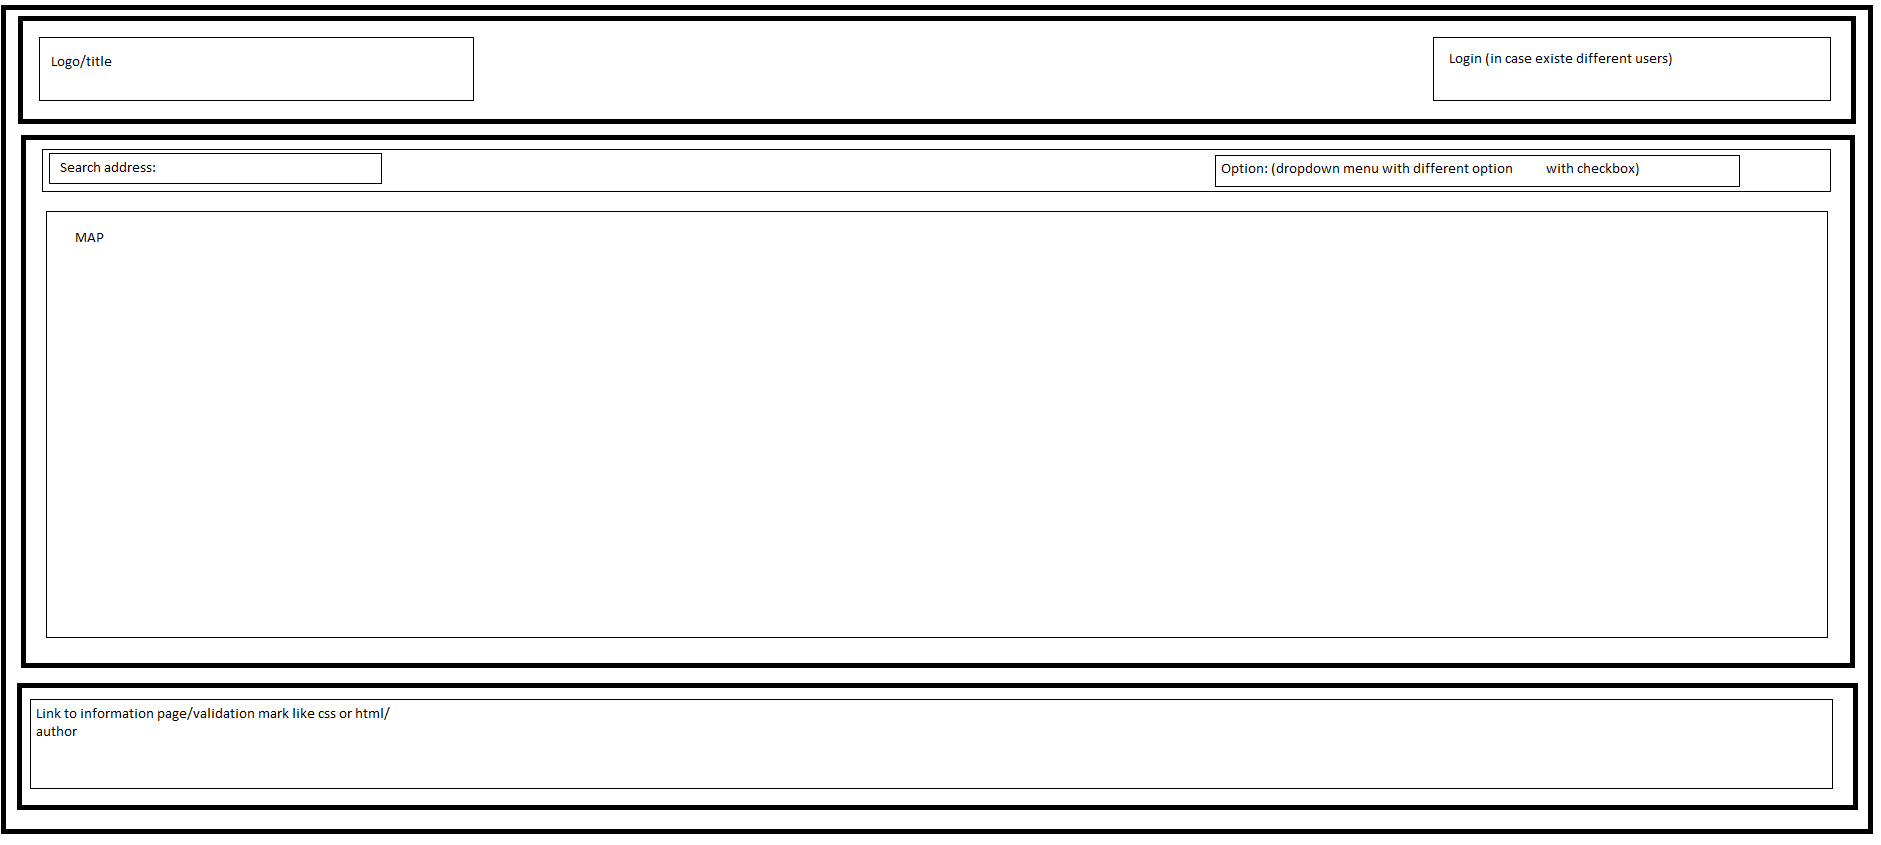
\includegraphics{../immagini/templateHtmlGDP.png}.\\
La sezione in alto individua un banner per il logo e login per gli utenti admin per effettuare modifiche alla mappa.
La sezione centrale visualizza la heat-map, una search bar per cercare il sito di assembramento che si vuole controllare e a lato di essa un menù per impostazioni di parametri aggiuntivi.\\
la sezione di footer sarà utilizzata per inserimento di informazioni sull'azienda proponente, il gruppo Jawa Druids e link per relativi ai propri siti web.